\documentclass{article}
\usepackage[utf8]{inputenc}
\usepackage[parfill]{parskip}
\usepackage{textcomp}
\usepackage{amsmath}
\usepackage{graphicx}
\usepackage[per-mode=symbol]{siunitx}
\usepackage{textgreek}
\usepackage{float}
\usepackage{qtree}
\usepackage{hyperref}

\usepackage[letterpaper,top=2cm,bottom=2cm,left=3cm,right=3cm,marginparwidth=1.75cm]{geometry}

\everymath{\displaystyle}

\title{APSC 259 written notes}
\author{Michael Ma}
\date{2021W1}

\begin{document}

\maketitle

\section{ATOMIC STRUCTURE}

The Bohr model attempts to consider spacing of electrons in atoms, as well as energy levels in each position.

The principal quantum number `n' can be an integer:

$n = 1, 2, 3 ...$
    
$    K, L, M ...$


The azimuthal number, $l$, tells about the shape of the orbital:

$l = 0, ..., (n-1)$

$l = 1, 2, 3, 4, ...$

$s, p, d, f$

Magnetic number, $m_e$, is number of electron orbitals in each subshell. For neutrals atoms, the orbitals are symmetrical. If electric/magnetic field is applied, then orbitals can deform. Magnetic number can be positive or negative.

Spin `$m_s$', the electrons can spin clockwise or counterclockwise. $m_s$ can be denoted +1/2 or -1/2. 

To fully describe an atom, we need $n$, $l$, $m_e$, and $m_s$.

Most engineering applications only $n$, $l$, and $m_e$ are sufficient.

Outer electrons are called valence

\subsection{ionic bonding}

Results in transfer of electrons from one atom to another

Positively charged ion is called cation

Negatively charged ion is called anion

The forces acting on the two atoms are influenced by coulomb force of attraction (electrostatic) as well as the repulsive force between the charged nuclei.

Coordination number is number of atoms an atom touches.
\begin{figure}[h!]
	\centering
	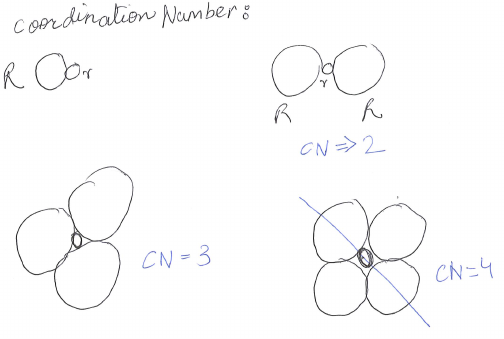
\includegraphics[width=0.66\textwidth]{assets/02394546.png}
	\caption{coordination number}
\end{figure}

\subsection{covalent bonding}
Word `covalent' comes from the cooperative sharing of valence electrons.
\begin{figure}[h!]
	\centering
	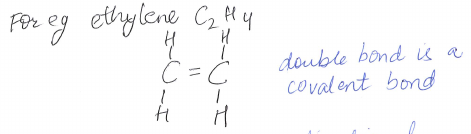
\includegraphics[width=0.66\textwidth]{assets/3173d297.png}
	\caption{Ethylene bonding}
\end{figure}

Covalent bonds are direction, and the ratio of atom sizes is less important.

Some bonds include linear bonds and tetrahedron config.

\begin{figure}[h!]
	\centering
	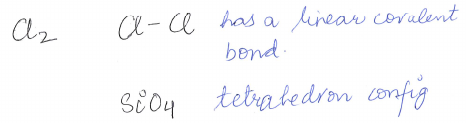
\includegraphics[width=0.66\textwidth]{assets/b1a91157.png}
	\caption{examples of linear and tetrahedron configs}
\end{figure}

\subsection{Metallic bond}
Represented as a ``cloud" or ``sea" of electrons.

\subsection{Secondary bonding}
When the electron cloud is not uniformly distributed then we have a dipole.

These materials have temporary dipoles, but these return to their neutral state when disturbance is removed (e.g. London dispersion forces in organic molecules).

\section{Crystal structure and crystallography}
A crystalline material must have a fundamental \underline{unit cell} which is releated in 3D throughout the material.

By calculating the lattice parameters, we can determine the size and shape of the unit cell.

\subsection{Body centred cubic (BCC)}
\begin{figure}[h!]
	\centering
	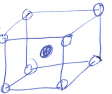
\includegraphics[width=0.66\textwidth]{assets/993a2f1f.png}
	\caption{BCC}
\end{figure}
Atoms located at the corners and one in the centre.

Side length of cube is: $a = \frac{4R}{\sqrt{3}}$

Coordination number of 8.

Number of inner atoms: 1

Number of corner atoms: $8\times\frac{1}{8} = 1$

Total number of atoms: 2

BCC is a relatively open structure.

\subsection{Face centred cubic (FCC)}
\begin{figure}[H]
	\centering
	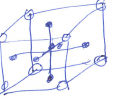
\includegraphics[width=0.66\textwidth]{assets/47a540f6.png}
	\caption{FCC}
\end{figure}

Atoms are located at the corners and in the faces of the sides.

Side length of cube is: $a = 2R\sqrt{3}$

Number of inner atoms: 0

Number of corner atoms: $8\times\frac{1}{8} = 1$

Number of face centred atoms: $6\times\frac{1}{2}=3$

Total number of atoms: 4

\subsection{hexagonal close packed (HCP)}

\begin{figure}[H]
	\centering
	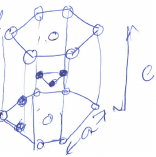
\includegraphics[width=0.66\textwidth]{assets/26287451.png}
	\caption{HCP}
\end{figure}

Hexagons attached on top of each other

Number of corner atoms: $12 \times \frac{1}{6} = 2$

Number of face atoms: $2\times \frac{1}{2} = 1$

Number of interior atoms: 3

$\frac{C}{a} = 1.633$

Coordination number of 12

\section{Density (sep 20)}

Knowing the number of atoms in each cell can enable us to calculate the theoretical density.

\begin{equation*}
    \rho = \frac{nA}{V_cN_A}
\end{equation*}

Where $n$ is number of atoms in a cell, $A$ is the atomic weight, $V_c$ is volume of the cell, and $N_A$ is Avogadro's number.

\subsection{Atomic packing factor}
\[\text{APF} = \frac{\text{Volume of atoms in the cell}}{\text{Total volume of cell}}\]

Density of a material is not the only important parameter in the mechanical strength of materials. Crystal orientation is also important.

To understand how a material will respond, we need to be ale to describe directions and planes inside a crystal.

\paragraph{Example} Rhodium has an atomic radius of 0.1345nm. The measured density is 12.41\si{\g\per\cubic\cm} and atomic weight is 102.91. Is this an FCC or BCC material?

\paragraph{answer} Assume it is FCC

for FCC: $n = 4, a = 2R\sqrt{2}, A = 102.91$

\begin{align*}
    \rho = \frac{nA}{a^3N_A}&=\frac{nA}{(2R\sqrt{2})^3N_A}\\
    &= \frac{4(102.91)}{(2(\num{1.325e-8})\sqrt{2})^3\cdot\num{6.022e23}}\\
    &=\SI{12.41}{\g\per\cm\cubed}
\end{align*}

Since our calculated density agrees with the measured density, then our assumption that Rh was FCC was correct!

\paragraph{Example} What is the APF of BCC crystal structure?

\paragraph{Answer} \begin{equation*}
    APF = \frac{V_s\text{(volume of atom)}}{V_c\text{(volume of cell)}}
\end{equation*}

For BCC, there are two atoms in each cell.

$V_s = 2\times\frac{4}{3} \pi R^3=\frac{8\pi R^3}{3}$

Volume of cell $=a^3$

For BCC, $a=\frac{4R}{\sqrt{3}}$

$V_c = \left(\frac{4R}{\sqrt{3}}\right)^3 = \frac{64R^3}{3\sqrt{3}}$

$APF = \frac{V_s}{V_c} = 0.68$

\section{Crystal directions and planes}

Directions for cubic crystals: [u v w]

To identify a specific direction, we need to determine the initial and final coordinates of the vector.

Starting point: $x_1, y_1, z_1$

end point: $x_2, y_2, z_2$

In crystallography we define directions in terms of multiple of coordinate axes:
\begin{align*}
    u&=n\left(\frac{x_2-x_1}{a}\right)\\
    v&=n\left(\frac{y_2-y_1}{b}\right)\\
    w&=n\left(\frac{z_2-z_1}{c}\right)
\end{align*}

For a unit lattice, $a=b=c$, and $n$ is an integer

In crystallography, do not use ``-1'', instead use ``$\overline{1}$''

\subsection{Directions for HCP crystals (sep 22)}
hexagonal system has [u, v, t, w]. Cubic uses [u, v, w].

\textit{\textless diagram\textgreater}

\begin{figure}[h!]
	\centering
	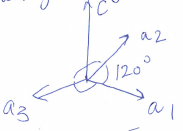
\includegraphics[width=0.66\textwidth]{assets/a6529061.png}
	\caption{angles and directions}
\end{figure}

\begin{table}[h!]
    \centering
    \begin{tabular}{ccc}
        \textbf{hex} & & \textbf{cubic} \\
        \hline
        \\
        $u$ & = & $\frac{1}{3}(2u-v)$\\
        \\
        $v$ & = & $\frac{1}{3}(2v-u)$\\
        \\
        $t$ & = & $-(u+v)$\\
        $w$ & = & $w$
    \end{tabular}
    \label{tab:conversionsfromhextocubic}
\end{table}

\subsection{Crystallographic Planes}
\begin{enumerate}
    \item Locate the origin of the cell
    \item Determine intercepts of plane within the unit cube
    \begin{itemize}
        \item Be careful of planes which are parallel to an axis
    \end{itemize}
    \item Find the inverse of the intercepts
    \begin{itemize}
        \item `$\infty$'
    \end{itemize}
    \item Multiply number to get integers (h, k, l) (Miller indices)
\end{enumerate}

\subsection{Miller-Bravais Index (sep 24)}
cubic\textrightarrow (h, k, l)

hexagonal\textrightarrow (h, k, i, l)

\begin{figure}[h!]
	\centering
	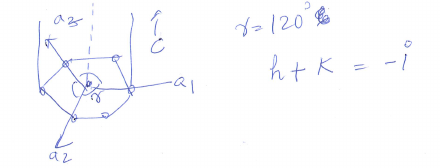
\includegraphics[width=0.66\textwidth]{assets/345e202b.png}
\end{figure}

\begin{figure}[h!]
	\centering
	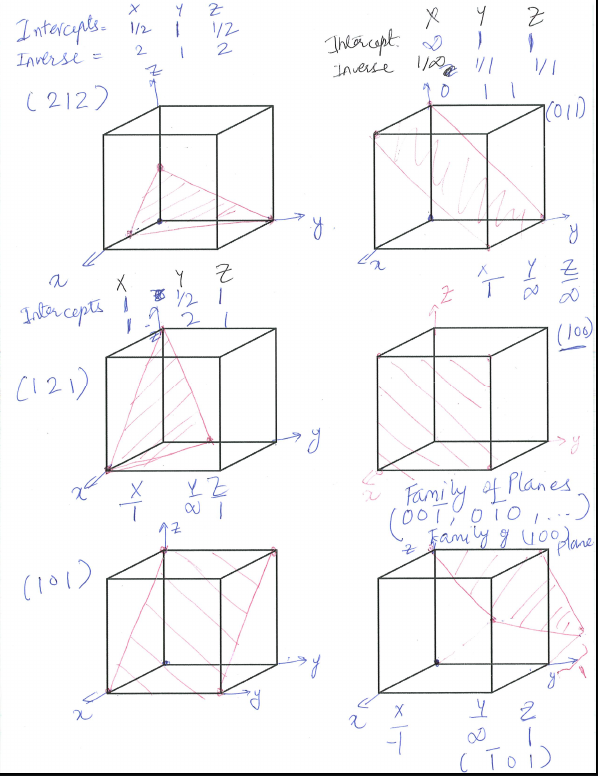
\includegraphics[width=0.66\textwidth]{assets/33eead8c.png}
	\caption{various plane intercepts}
\end{figure}

\begin{figure}[h!]
	\centering
	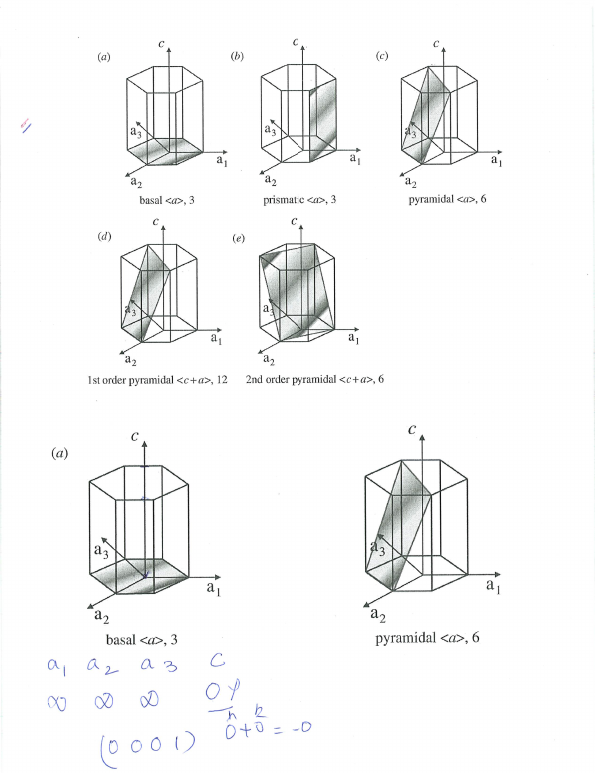
\includegraphics[width=0.66\textwidth]{assets/71838378.png}
	\caption{hex planes}
\end{figure}

\subsection{Crystal Density}
The crystal as they form may contain planes with high planar or linear density.

$\text{Linear Density (L.D.)} = \frac{\text{number of atoms in a specific direction}}{\text{length of the direction}}$

$\text{Planar Density (P.D.)} = \frac{\text{number of atoms on a plane}}{\text{area of the plane}}$

This is important for bonding. The denser the plane, the stronger the bond.

\subsubsection{X-ray diffraction (XRD)}
Diffraction - similar to rocks skipping on the surface of water.

This can be done with x-rays but also electrons and neutrons.
\begin{figure}[h!]
	\centering
	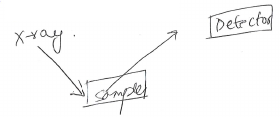
\includegraphics[width=0.66\textwidth]{assets/4e47d9c5.png}
	\caption{rough sketch of XRD}
\end{figure}

`\textlambda'-wavelength

The type of radiation would determine the `\textlambda' of the beam

Depending on the material, the spacing between the crystal planes (d-spacing) will vary.

\paragraph{Bragg's law} $n\lambda=2d\sin(\theta)$

$n$ is usually equal to 1, and $\theta$ is the diffraction angle.
\begin{figure}[h!]
	\centering
	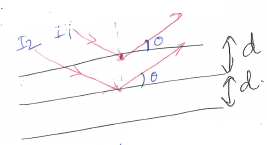
\includegraphics[width=0.66\textwidth]{assets/7e865405.png}
	\caption{diffraction}
\end{figure}

The d-spacing between plaes is unique for different materials. We can relate this to the size of a crystal:
\begin{align*}
    \text{FCC/BCC: } d_{hkl} &= \frac{a}{\sqrt{h^2+k^2+l^2}}\\
    \Rightarrow d_{1 1 0} &= \frac{a}{\sqrt{1^2+1^2+0^0}}\\
    &= \frac{a}{\sqrt{2}}\\
    \text{HCP: } \frac{1}{d^2} &= \frac{4}{3}\left(\frac{h^2+hk+k^2}{a^2}\right)+\frac{l^2}{c^2}
\end{align*}

For BCC, h+k+l (even number)

Only then (h k l) plane will reflect.

For FCC, h k l all odd or even

% This is when I started taking LaTeX notes

\section{STACKING SEQUENCES (where these LaTeX notes originally started}
FCC: ABC ABC ABC ...

HCP: AB AB ...

Depending on how planes stack (or are oriented) with respect to each other we assign them a label.\\
If the planes are positioned directly on top of each other (simple cubic)\\
\[\rightarrow A\ A\ A\]

\section{MECHANICAL PROPERTIES OF METALS}
The response of a metal to an external stimulus is crucial in determining how a part will perform in service.\\ 
Brittleness \textrightarrow\ Tendency to fracture when a small load is applied, e.g. glass, ceramic tiles\\

Ductility \textrightarrow\ How much a material can deform without sustaining internal damage\\

Creep \textrightarrow\ deformation of a material at high temperature.\\

Fatigue \textrightarrow\ weakening of a material due to repeated (or cycling) loading.\\

Elasticity \textrightarrow\ Ability of a material to return to its original shape.\\

Plasticity \textrightarrow\ Ability of a material to stay deformed after the external force is removed.

Hardness $\rightarrow$ Ability to resist permanent change in shape.

Resilience: Ability to absorb energy and resist impact loadings.

Stiffness: Ability of a metal to resist additional deformation when loading continues.

Toughness: Ability of a metal to resist fracture.

To quantify these parameters \& properties, standard societies have developed common procedures to ensure consistency of the results. In Canada, ASTM standards are used.

\begin{figure}[h!]
	\centering
	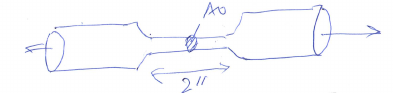
\includegraphics[width=0.66\textwidth]{assets/12c51b4a.png}
	\caption{Dogbone being stretched, showing the location of $A_0$}
\end{figure}
\[A_0 = \text{original cross sectional area}\]

\[\textrm{Engineering stress} = \sigma = \frac{F}{A_0}\]

\[\textrm{Engineering Strain: } \epsilon\]

\[\epsilon = \frac{l_i - l_0}{l_0} = \frac{\Delta l}{l}\]

Where $l_0$ is initial length, and $l_i$ is instantaneous length.

Note: $\epsilon$ has no unit, but many textbooks refer to it as in/in or m/m

The tensile engineering stress \& strain equations can also be used for compressive tests.

\subsection{Shear and torsion}

\begin{figure}[h!]
	\centering
	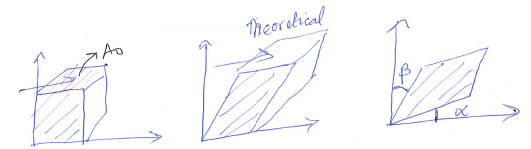
\includegraphics[width=0.66\textwidth]{assets/df560772.png}
	\caption{Diagrams of shear}
\end{figure}

Shear strain = $\gamma = x + \beta$

Shear stress $\tau = \frac{F}{A_0}$

If you are not deforming the material by tensile/compression or shear, then we call it torsion.

\subsection{Elastic Deformation}

During the initial stage of deformation, the stress experienced by the material proportional to the deformation strain.

\[\textrm{Hooke's Law: } \sigma = E \epsilon\]

$\sigma$ is stress, $E$ is Young's Modulus, $\epsilon$ is strain.
    
In the elastic region, $E$ = constant.

The higher the value of $E$ the stiffer the material. 

The temperature of a material has a significant impact on $E$.

Secants/tangents are used for materials which do not have a linear stress-strain relationship.

A similar relationship could be written for shear deformation:

\[\tau = G \gamma\]

$G$ is shear modulus, $\gamma$ is shear strain, $\tau$ is shear stress.

In elastically behaving materials, the tensile force in the z-direction causes strain $\epsilon_z$. 

This causes contraction in the perpendicular directions $\epsilon_x, \epsilon_y$

For isotropic materials, we can use Poisson's ratio to relate strains

\[\nu = \frac{-\epsilon_x}{\epsilon_z} = \frac{-\epsilon_y}{\epsilon_z}\]

This ratio can relate E and G:

\[E = 2G(1+\nu)\]

\subsubsection{Example}
A titanium wire is used in medical implants. It has a diameter of 3 mm and is 30 mm long. For Ti, $E$ = 107 GPa. Calculate the theoretical elongation if a 500N Force is applied. Assume all load is elastic.

\[\epsilon = \frac{\Delta l}{l_0}\]
\[\Delta l = \epsilon l_0 = l_0 \frac{\sigma}{E} = l_0\frac{1}{E} \cdot \frac{F}{A_0}\]
\[l_0\frac{1}{E} \cdot \frac{F}{\pi (\frac{d_0}{2})^2} = \frac{4l_0 F}{E\pi d_0^2}\]
\[\Delta l = \frac{4(30 \times 10^{-3})500}{(107\times 10^9)\pi (3\times10^-3)^2} = 0.02 \si{\mm}\]

isotropic: Properties are the same regardless of direction.

anisotropic: Properties are different in different directions.

\subsubsection{Example}

A cylindrical spaces in a circuit board is compressed during board assembly. Initially it was 20 mm in diameter but after compression it is 20.025 mm. The final length is 74.96 mm. What is/was the original length?

$E = 105 \text{ GPa}$, $G = 39.7\text{ GPA}$

\subsubsection*{answer}

$\epsilon_x = \frac{\Delta d}{d_0} = \frac{20.025 - 20}{20} = 1.25 \times 10^{-3}$

$\nu = \frac{E}{2G} = \frac{105 \times 10^9}{2(39.7 \times 10^9)} -1 = 0.322$

$some shit$

$l_0 = 75.25\si{\milli\metre}$

\subsection{Plastic deformation}

Many materials can exhibit elastic response up to about 0.5\%. Above this strain, the material will being to permanently change and permanent deformation will occur.

\begin{figure}[H]
	\centering
	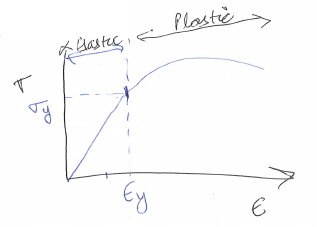
\includegraphics[width=0.66\textwidth]{assets/8cadff62.png}
	\caption{The permanent deformation is the result of dislocation movement}
\end{figure}

\subsection{Yielding (or Yield Point) or (flow stress)}

Transition from elastic to plastic regime

You do not want to approach this value.

\begin{figure}[H]
	\centering
	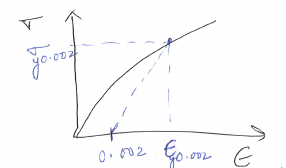
\includegraphics[width=0.66\textwidth]{assets/83f7972e.png}
	\caption{Yield strength graph}
\end{figure}

For many materials, it is not easy to find the yield point

We found an offset ``0.002'' offset. The stress at offset ``$\sigma_{y0.002}$''

\subsection{Tensile Strength}

As load continues to rise, the material keep deforming. At UTS (Ultimate Tensile Strength), the material will experience ``fatal'' void formation.

\textrightarrow The voids merge and cracks develop

\textrightarrow Because the material is being deformed in plastic regime, the damage in material continues

$\star$ The load required to continue deforming the material reduces after UTS.

\begin{figure}[H]
	\centering
	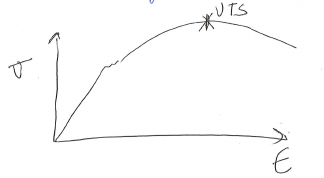
\includegraphics[width=0.66\textwidth]{assets/a9d11a8c.png}
	\caption{Ultimate tensile strength on a stress-strain diagram}
\end{figure}

Fracture: The last point of the stress-strain diagram when the material can sustain any load.

Ductility: The measure of deformation a material can take before fracture. The more deformation we have before fracture occurs, the more warning we have.

% ductile material image
\begin{figure}[h!]
	\centering
	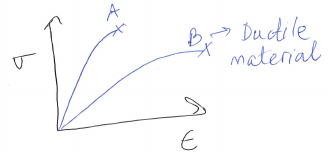
\includegraphics[width=0.66\textwidth]{assets/2160dc14.png}
	\caption{Ductile material stress-strain graph}
\end{figure}

\% Elongation = $(\frac{L_f - L_0}{L_0})\times 100\%$

$L_f$ = elongation of fracture

$L_0$ = original length

\% reduction in area = $(\frac{A_0 - A_f}{A_0})\times 100\% $

\subsection{RESILIENCE}
The amount of energy in the elastic region

%area under curve graph
\begin{figure}[H]
	\centering
	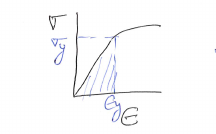
\includegraphics[width=0.66\textwidth]{assets/9cb7c396.png}
	\caption{Resilience graph ($U_r$)}
\end{figure}
$U_r = \frac{1}{2}\sigma_y\epsilon_y \Rightarrow \frac{1}{2} \frac{\sigma_y^2}{E}$

\subsection{TOUGHNESS}
The amount of energy that can be absorbed by fracture. No formula.
% toughness graph
\begin{figure}[h!]
	\centering
	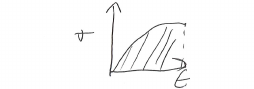
\includegraphics[width=0.66\textwidth]{assets/f2e471df.png}
	\caption{Toughness graph}
\end{figure}

\subsection{TRUE STRESS AND TRUE STRAIN}

$\sigma_T = \frac{F}{A_i}$, $A_i$ = instantaneous area

$\epsilon_T = \ln(\frac{l_i}{l_0})$

The true and engineering stress/strain can be related:

$\sigma_T = \sigma(1+\epsilon)$

$\epsilon_T = \ln(1+\epsilon)$

$\star \epsilon$ is not percentage

\subsubsection{Strain hardening}
The deformation in materials can become harder due to strain hardening. This instantaneous change will affect the $\sigma-\epsilon$ diagram.

$\sigma_T = K(\epsilon_T)^n$

where $n$ is the strain hardening exponent, and $K$ is a constant

% n = 10 and n = 2 graph
\begin{figure}[h!]
	\centering
	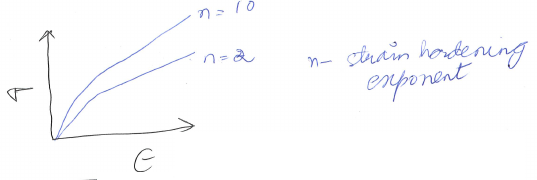
\includegraphics[width=0.66\textwidth]{assets/1aa4dbd7.png}
	\caption{Strain hardening}
\end{figure}

\subsection{Class example}

\paragraph{Q1: Calculate Modulus of Elasticity 'E'}

\begin{equation*}
\begin{split}
    E &= \frac{\Delta\sigma}{\Delta\epsilon}\\
    &= \frac{200-0}{0.00125-0} \\
    &= 160 000 \si\MPa = 160 \si\GPa
\end{split}
\end{equation*}

\paragraph{Q2: Yield strength at a strain offset of 0.002:}

From the stress-strain diagram($\sigma-\epsilon$):

$\sigma_0.002 \approx 285 \si\MPa$

\paragraph{Q3: Ultimate Tensile Strength (UTS)}

UTS from the graph: 405 \si\MPa

\paragraph{Q4: Ductility of allow at fracture} Ductility is the amount of plastic strain

$0.18 - 0.0015 = 0.1785 = 17.85\%$

\begin{figure}[h!]
	\centering
	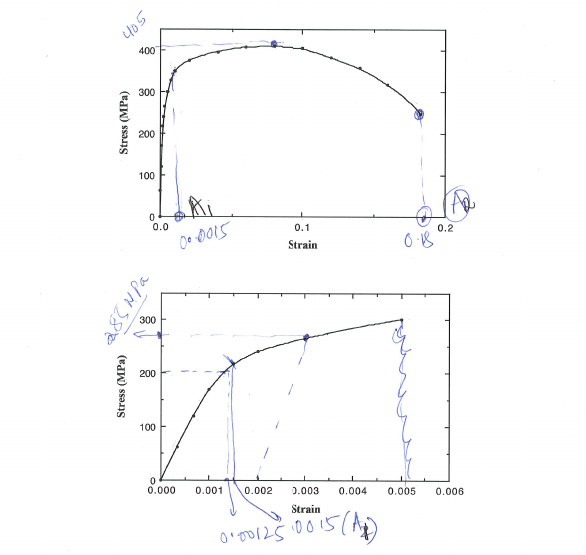
\includegraphics[width=0.66\textwidth]{assets/9840bbbf.png}
	\caption{more graphs}
\end{figure}

\paragraph{Q5: Find the modulus of Resilience}

\begin{displaymath}
U_r = \frac{\sigma_y^2}{2E} = \frac{285^2}{2(160)\times10^3} = 0.25\si{\MN\per\m\squared}
\end{displaymath}

\section{Hardness}

This test provides a measure of the response of a material to an external load.

\subsection{Rockwell test ``HR"}

\begin{itemize}
    \item Consist of a machine that applies a compressive load onto a material
    \item Depth of the indentation is a measure of the material's hardness
\end{itemize}

\subsubsection{Test procedure}

\begin{enumerate}
    \item Preload and set a reference depth
    \item load
    \item remove load, measure depth
\end{enumerate}

\subsubsection{Rules}

\begin{enumerate}
    \item Stay away from the sample edges, about 10 times your indentation diameter
    \item Stay away from other hardness measurement locations, about 3 times your indentation diameter
\end{enumerate}

\subsection{Brinell Hardness Test ``HB''}

\begin{itemize}
    \item uses a steel ball to indent the material
    \item measure diameter of indentation
\end{itemize}

Tensile strength = 3.45 HB (\si\MPa)

Tensile strength = 500 HB (psi)

\subsection{Vickers Hardness ``HV"}

\begin{itemize}
    \item Microhardness measurement with a diamond indentor
    \item We measure the size of the indents
\end{itemize}

\begin{figure}[h!]
	\centering
	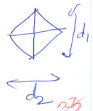
\includegraphics[width=0.26\textwidth]{assets/e44ed62b.png}
	\caption{Vicker's hardness diamond}
\end{figure}

\subsection{Fatigue}

Fatigue is a type of material failure where the material fails below its yield strength, because of cyclic loading.

The damage in the material accumulates over time and may not be visible, failure occurs in a brittle fashion, even if the material is ductile.

% fatigue sine wave graph
\begin{figure}[h!]
	\centering
	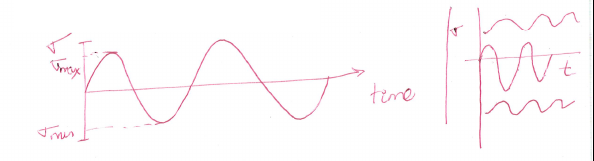
\includegraphics[width=0.66\textwidth]{assets/76631775.png}
	\caption{Cyclic loading as a sine wave}
\end{figure}

$\sigma_{mean} = \frac{\sigma_{max} + \sigma_{min}}{2}$

Stress range $= \sigma_r = \sigma_{max} - \sigma_{min}$

Amplitude $= \frac{\sigma_r}{2}$

Stress ratio $= R = \frac{\sigma_{min}}{\sigma_{max}}$

% stress-no. of cycles graph
\begin{figure}[h!]
	\centering
	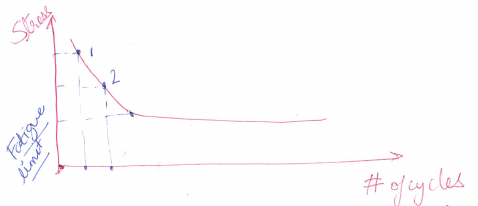
\includegraphics[width=0.66\textwidth]{assets/d31ee76a.png}
	\caption{Stress-number of cycles graph}
\end{figure}

$\star$ The fatigue behaviour of a material can be evaluated using standard tension/compression tests or rotary fatigue tests.

$\star$ In both cases we count the number of cycles until failure. This gives us the ``S-N curve."

$\star$ At or below the fatigue limit, the material does not break.

Fatigue strength: slices after $10^7$ cycles

Fatigue life: number of cycles required to fracture at a given load.

\subsubsection{How to reduce fatigue damage:}

\begin{enumerate}
    \item Eliminate sharp corners
    % insert pictures of square penis
    \item Compressive residual stresses
    \item Surface treatments, e.g. hardening
\end{enumerate}

\subsection{Creep}

The deformation of materials, usually at elevated temperatures. $\sim 0.4$ Tm

When a material is heated/loaded, it will experience strain as a factor of time.

%creep graph
\begin{figure}[h!]
	\centering
	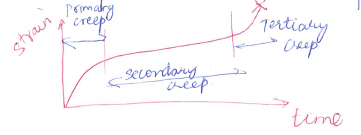
\includegraphics[width=0.66\textwidth]{assets/896dccb9.png}
	\caption{Creep graph}
\end{figure}

Primary: initial deformation

Secondary: steady state

Tertiary: accelerated deformation loading to rupture

``Time to rupture'': time to reach failure

The stress and temperature have the most significant impact on creep.

Steady state: $\dot{\epsilon_s} = k_1 \sigma^n (k_1 n \rightarrow \text{constant})$

If temperature is changing:
\begin{equation*}
    \dot{\epsilon_s} = k_2 \sigma^n e^{\frac{-Q}{RT}} (Q \text{ is activation energy})
\end{equation*}

\section{Material failure (Oct 15)}

A material will lose its strength and fully (or partially) separate into multiple pieces.

Failure can occur due to a variety of factors:
\begin{itemize}
    \item tension
    \item compression
    \item shear
    \item torsion
    \item heat
    \item pressure
\end{itemize}
All of the above can be a ductile or brittle failure.

During loading of a material, it will experience stress which is ale to initiate a crack. Additional loading will allow the crack to grow and propagate.

\subsection{Ductile fracture}

$\rightarrow$ A material experiences a lot of \underline{plastic} deformation.

$\rightarrow$ In metals, a necking phenomenon is an indication of plastic deformation.

% insert necking image
\begin{figure}[H]
	\centering
	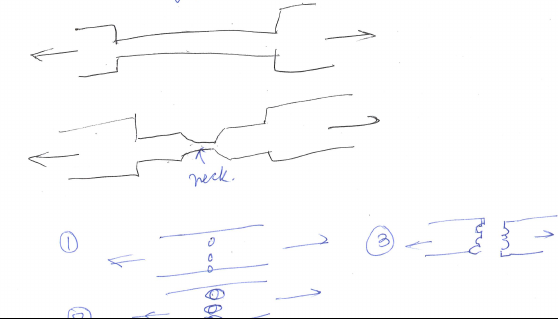
\includegraphics[width=0.66\textwidth]{assets/286897da.png}
	\caption{Necking and elliptical holes in a fracture}
\end{figure}

% cone cup fracture
\begin{figure}[h!]
	\centering
	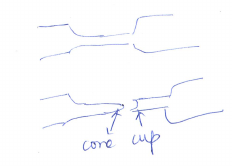
\includegraphics[width=0.66\textwidth]{assets/61ecd582.png}
	\caption{Cone and cup fracture}
\end{figure}

Depending on the amount of plasticity a material can handle, the necked region can experience a cone-and-cup fracture.

\subsection{Brittle fracture}
\begin{itemize}
    \item Very little stretching/plastic deformation
    \item Fracture happens rapidly without warning
\end{itemize}

% brittle fracture diagram
\begin{figure}[h!]
	\centering
	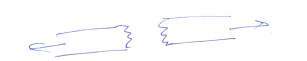
\includegraphics[width=0.66\textwidth]{assets/ae4c2aa2.png}
	\caption{Brittle fracture}
\end{figure}

\subsection{Grains}
% grains diagram
\begin{figure}[h!]
    \centering
    \includegraphics{}
    \caption{Grains arrangement in materials}
    \label{fig:grains}
\end{figure}

The racks can propagate along the grain boundaries.

% integranular fracture diagram
\begin{figure}[h!]
	\centering
	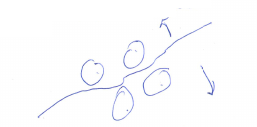
\includegraphics[width=0.66\textwidth]{assets/80de7856.png}
	\caption{Intergranular fracture}
\end{figure}

Also, cracks can propagate through grains.

% transgranular fracture diagram
\begin{figure}[h!]
    \centering
    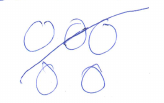
\includegraphics[width=0.66\textwidth]{assets/044358e4.png}
    \caption{Transgranular fracture}
    \label{fig:tg_fracture}
\end{figure}

\paragraph{Question} How do we know when a material will fail (fracture mechanics)?

The fundamental concept is based on the fact that materials will have a flaw or defect.

% the fucking tree diagram and some diagram with rho_t
\Tree[.{Stress concentration} 
        [.{geometry of the part} ]
        [.{voids} ]
        [.{Inclusion/imperfections} ]]

\begin{figure}[H]
	\centering
	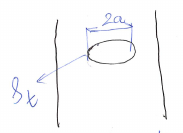
\includegraphics[width=0.66\textwidth]{assets/b384fde4.png}
	\caption{Stress of material with hole (I think)}
\end{figure}

The max stress that can occur at a crack tip is:
\begin{equation*}
    \displaystyle \sigma_m = 2\sigma_0 \left(\frac{a}{\rho_t}\right)^{\frac{1}{2}}
\end{equation*}

$\sigma_0$: applied stress

$\rho_t$: radius of curvature

$a$: crack length

$\star$ The sharper the tip of the crack, i.e. the smaller the $\rho_t$ value, the higher stress magnification will be.

We can estimate the stress concentration factor:
\begin{equation*}
    K = \frac{\sigma_m}{\sigma_0} = 2\left(\frac{a}{\rho_t}\right)^{\frac{1}{2}}
\end{equation*}

\subsection{Fracture toughness}

The stress required to propagate a crack $\sigma_c$ and the crack has a length $a$:
\begin{align*}
    K_c &= y\sigma_c \sqrt{\pi a}, y \text{ constant }\\
    \sigma_c &= \sqrt{\frac{2E\gamma_s}{\pi a}}, \gamma_s \text{surface energy}
\end{align*}

There is a special scenario where the \underline{thickness of the material} is much bigger than the crack size.

Plane strain situation $\rightarrow K_{Ic}$

\begin{equation*}
    K_{Ic} = y\sigma\sqrt{\pi a}, \sigma \text{ applied stress}, y \textrm{ constant}
\end{equation*}

\subsection{some question (Oct 18)}

\begin{enumerate}
    \item If the specific surface energy for soda-lime glass is $0.3 \si{J/m^2}$, using data given, compute critical stress required for propagation of a surface crack of length 0.05\si{mm}.
    
    E = 69 GPa
    
    \paragraph{Answer} 
    \begin{align*}
        \sigma_c &= \left(\frac{2E\gamma_s}{\pi a}\right)^{\frac{1}{2}}\\
        &= \frac{2\times 69\times 10^9 (0.30)}{\pi(0.05\times10^{-3}\si\m)}\\
        &= 16.2 \times 10^6 \si{N/m^2}\\
        &= 16.2 \si\MPa
    \end{align*}
\end{enumerate}

\section{Imperfections}


\section{Grain size example:}
For an ASTM grain size of 8, approximately how many grains will be per square inch at a magnification of 100x?

\paragraph{Answer} $n = 2^{G-1} = 2^{8-1} = 128 \text{ grains/in}$

What if we don't use a microscope with 100x magnification, but we just look with naked eye?

\begin{align*}
    n_M \times \left(\frac{M}{100}\right)^2 &= 2^{G-1}\\
    M &= 1\\
    n_1\left(\frac{1}{100}\right)^2 &= 2^{8-1}\\
    n_1 &= 1280000 \text{ grains/in}^2
\end{align*}

\section{Diffusion (Oct 22 EVERYTHING FROM HERE ON OUT NOT ON MIDTERM)}

Two options:
\begin{enumerate}
    \item Liquid or solid diffusion with intermixing of two materials
    \item Self-diffusion (e.g., H2O molecules moving inside of a water glass)
\end{enumerate}

Examples include smelling coffee in a room, sugar diffusing in tea, biological diffusion, and helium balloons diffusing.

\subsection{Fick's first law}

Steady state is when rate of diffusion in is same as rate out

$J_x = -D\frac{\partial c}{\partial x}$

Where $J_x$ is flux (or flow rate) of diffusion species in the x-direction due to a concentration gradient

$D$ is the diffusion constant aka diffusivity

\subsection{Fick's second law}

$\frac{\partial c_x}{\partial t} = \frac{\partial }{\partial x}\left(D\frac{\partial c_x}{\partial x}\right)$

If we assume a semi-infinite solid, with a surface concentration of the diffusing species, $c_s$, constant, then we can solve using

$\frac{c_x-c_0}{c_s-c_0} = 1 - erf\left(\frac{x}{2\sqrt{Dt}}\right)$

where $x$ is position of interest, $t$ is time of interest, $c_0$ is initial bunk concentration, $c_s$ is surface concentration.

\subsection{Effect of temperature}

$D = D_0 e^{\frac{q}{kT}}$

Where $D_0$ is constant, q is activation energy

% temp graph
\begin{figure}[h!]
	\centering
	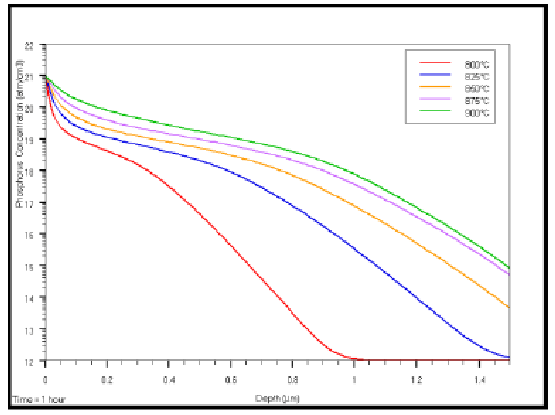
\includegraphics[width=0.66\textwidth]{assets/30d8dd09.png}
    \caption{Temperature graph}
    \label{fig:temp}
\end{figure}

\subsection{Diffusion rates}

Fastest is surface, e.g. catalytic converters, photographic film

Medium is grain boundary, critical for durability in microelectronics

Slowest is bulk(volume)

\subsection{Fick's first law (steady state) example}
A steel plate 1.5 mm thick has a N$_2$ atmosphere on one side at 1200$^\circ$C. The plate has been at this state long enough so that steady state was established. The diffusion constant/coefficient for N$_2$ into steel at this temperature is 6 $\times$ 10$^{-11}$ m$^2$/s and the diffusion flux is 1.2 $\times$ 10$^{-3}$ kg/m$^2$s. The concentration of N$_2$ on one side is 4 kg/m$^3$. How far into the sheet do we need to go to reach a concentration of 2 kg/m$^3$?

% screenshot of solution here

\paragraph{Q} Determine the carburizing time necessary to achieve a carbon concentration of 0.45\% at a position 2mm into an iron-carbon alloy that initially contains 0.20 wt\% C. The surface concentration is to e maintained at 1.30 wt\% C and the treatment is to be conducted at 1000$^\circ$C. Assume $D = \num{1.93e-11}$\si{\metre\squared\per\second}.

% answer here
\begin{figure}[h!]
	\centering
	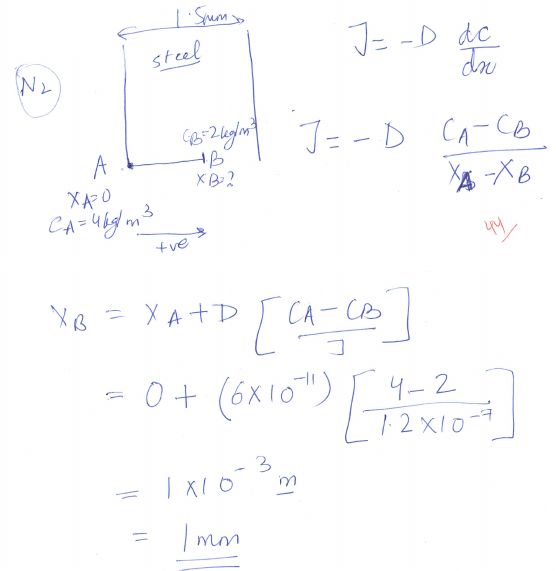
\includegraphics[width=\textwidth]{assets/c547ceac.png}
	\caption{Too lazy to write out the answer, so here is a screenshot}
\end{figure}

\paragraph{Q(Oct 25)} A FCC-ion carbon alloy containing 0.35 wt\% C is exposed to an $O_2$ rich and virtually carbon free atmosphere at 1400K ($112.7^\circ$ C). Under these circumstances, the C diffuses from the alloy and reacts at the surface with the $O_2$ in the atmosphere; that is, the C concentration at the surface position is maintained at 0 wt\% C. At what position will the C concentration be 0.15 wt\% after 10-h treatment. D at 1400K = \num{6.9e-11}\si{\metre\squared\per\second}

\paragraph{Answer}
\begin{align*}
    \frac{C_x - C_0}{C_s - C_0} &= 1 - erf\left(\frac{x}{2\sqrt{DT}}\right)\\
    \frac{0.15-0.35}{0-0.35} &= 1-erf\left(\frac{x}{2\sqrt{DT}}\right)\\
    0.5714 &= 1-erf\left(\frac{x}{2\sqrt{DT}}\right)\\
\end{align*}

\begin{table}[h!]
    \centering
    \begin{tabular}{c c}
        $Z = 0.4$ & $erf(Z) = 0.4284$\\
        $Z = ?$ & $erf(Z) = 0.4286$\\
        $Z = 0.45$ & $erf(Z) = 0.4755$
    \end{tabular}
    \caption{Values of Z from table}
    \label{tab:Zvalues}
\end{table}

\begin{align*}
    \frac{Z-0.4}{0.45-0.4} &= \frac{0.4286 - 0.4284}{0.4755-0.4284}\\
    Z &= 0.4002\\
    \frac{x}{2\sqrt{DT}} &= 0.4002\\
    \frac{x}{2\sqrt{(\num{6.9e-11})10\times60\times60}} &= 0.4002\\
    x &= \num{1.26e-3}\si{\metre}
\end{align*}

\section{Phase diagrams (Nov 1)}

In real life, we rarely use pure materials. Materials could be ``99.9\%'' pure, this is called ``3N'', or Three nines.

4N and 5N purities are 99.99\% and 99.999\%, respectively. Little bit more expensive.

High tech: 6N and 7N, high purity and really fucking expensive.

Alloys are mixtures of elements. Depending on the composition of the alloy ``everything'' changes.
\begin{itemize}
    \item mechanical properties
    \item optical properties
    \item electrical properties
    \item chemical properties
\end{itemize}

Dissolution of elements in each other depends on the concentration and temperature

We can form \underline{phases} and \underline{chemistries} which are unique for a given combination of temperature, pressure, and concentration:

\begin{itemize}
    \item Liquid solution: Mix solute in small quantity and solvent (matrix)
    \begin{description}
    \item[solute:] intersticial/substitutional atoms
    \item[solvent:] matrix
    \end{description}
    
    \item Solid solution: mixing of solids or reactions in solids which produce new compounds.
\end{itemize}

$\star$ The amount of how much solute can be dissolved in a solvent is dependent on temperature and pressure and is termed as solubility limit.

The graph of temperature vs composition is called as a phase diagram.

Phase: can be chemically or physically separated.

Phase diagram for 1 element: Uniary phase diagram

for 2 elements: binary phase diagram

for 3 elements: tertiary phase diagram

\begin{figure}[h!]
	\centering
	\includegraphics{}
	\caption{Carbon phase diagram}
\end{figure}

\begin{figure}[h!]
    \centering
    \includegraphics{}
    \caption{water?}
    \label{fig:my_label}
\end{figure}

\begin{figure}[h!]
    \centering
    \includegraphics{}
    \caption{Thallium diagram}
    \label{fig:my_label}
\end{figure}

\begin{figure}[h!]
    \centering
    \includegraphics{}
    \caption{sugar}
    \label{fig:my_label}
\end{figure}

\paragraph{Editor's note:} \textit{I am sure the above diagrams were shown in lecture, but I cannot find them.}

\paragraph{(Nov 3)} The diagrams that we see in many textbooks are ``equilibrium'' phase diagrams.
\begin{itemize}
    \item It has been at the state for a long time.
    \item When time is insufficient to achieve equilibrium, then the solubility lines will shift.
\end{itemize}

\paragraph{Terms (Cu-Ni system): }
\begin{itemize}
    \item Liquid: liquid mixture of Cu and Ni
    \item Solid solution: marked with lowercase Greek letters ($\alpha$, $\beta$, $\gamma$)
\end{itemize}

\subsection{Phase boundaries}

liquidus line: the material becomes liquid above this line.

solidus line: the material becomes solid below this line.

Pure elements: `Tm', melting point of pure element

Phase transformation: liquid to (liquid + solid), (liquid + solid) to liquid

What do we get out of a PD?
\begin{enumerate}
    \item Which phases are present at which temperature, pressure, and concentration combinations
    \item Composition of a phase
    \item Weight fraction of each phase
\end{enumerate}

\subsubsection{Phases present}

\paragraph{Q} Locate the temperature/composition on the PD and read off the phase that exists at that point.

\paragraph{A} Alloy with 28\% wt Ni 

\begin{enumerate}
    \item $@1300\si\celsius$: All liquid
    \item $@1200\si\celsius$: combination of $\alpha$ and L
    \item $@1000\si\celsius$: All solid($\alpha$)
\end{enumerate}

\subsection{Phase composition (concentration)}

\begin{figure}[H]
	\centering
	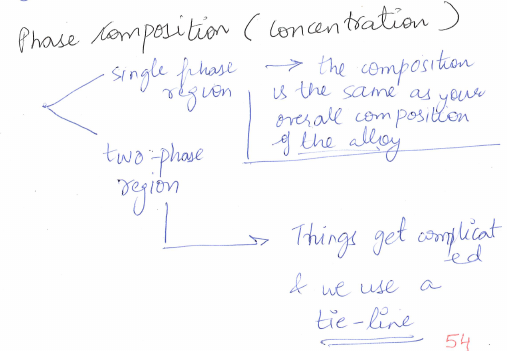
\includegraphics[width=0.66\textwidth]{assets/759b1bb4.png}
	\caption{Phase composition (concentration)}
\end{figure}

\begin{figure}[h!]
	\centering
	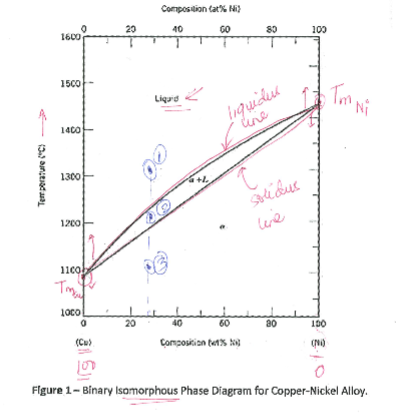
\includegraphics[width=0.60\textwidth]{assets/aad184f6.png}
	\caption{Binary isomorphous phase diagram for Cu-Ni alloy}
\end{figure}

\begin{figure}[H]
	\centering
	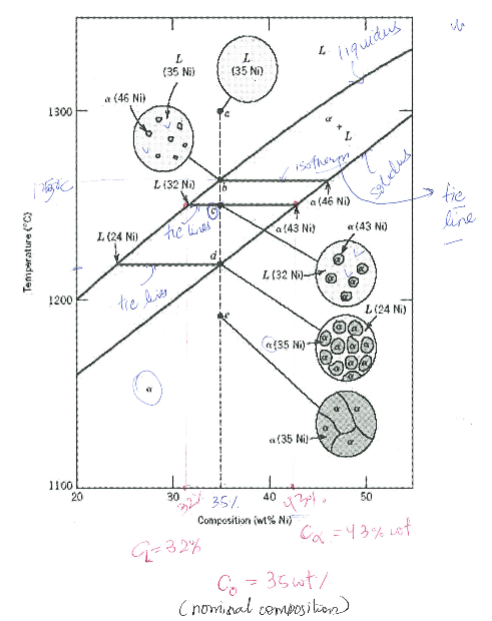
\includegraphics[width=0.60\textwidth]{assets/1149aa48.png}
	\caption{grains and shit}
\end{figure}

In the two phase region, to find the composition:
\begin{enumerate}
    \item Select the temperature of interest in the two phase-region
    \item Write the concentration values where the tie line intersects the boundaries
    \item locate your overall composition
\end{enumerate}

\subsection{Weight fraction (Nov 5)}

How much of a phase is present at a given temperature/concentration

\subsubsection{DETERMINATION OF PHASE AMOUNTS}

Single phase region: the amount of phase is 100\%

Two-phase region: Inverse lever rule

\subsubsection{Procedure for the inverse lever rule:}

\begin{enumerate}
    \item Construct a horizontal tie line
    \item On the tie line, mark the composition of your alloy
    \item Determine the overall length of the tie line
    \item Fractions of phases are related to the opposite segment on the tie-line with respect to the composition of the alloy
\end{enumerate}
*At point C, what is the weight fraction of `L' and `$\alpha$' (Linear interpolation):

\begin{figure}[H]
	\centering
	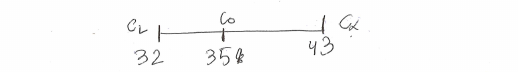
\includegraphics[width=0.66\textwidth]{assets/ccd151c8.png}
\end{figure}

$w_\alpha = \displaystyle\frac{35-32}{43-32} = 0.27 = 27\%$

$w_L = 100-27=73\% \Rightarrow \frac{C_\alpha-C_0}{C_\alpha-C_L}$

\subsubsection{Binary eutectic phase diagrams}

\begin{figure}[h!]
	\centering
	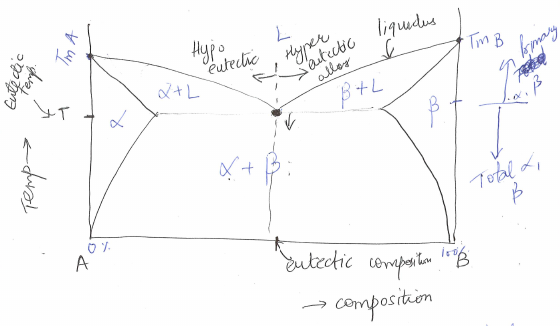
\includegraphics[width=0.66\textwidth]{assets/89ccf715.png}
	\caption{Binary eutectic phase diagram}
\end{figure}

At the eutectic temperature and concentration \textalpha, \textbeta, and $L$ exist in equilibrium at the same time. 

The phase (\textalpha, \textbeta) which is present at the eutectic temperature is called eutectic(\textalpha\textbeta)
\begin{itemize}
    \item primary $\alpha = \alpha'$
    \item eutectic $\alpha = \alpha_e$
    \item total $\alpha = \alpha_T$
\end{itemize}

\begin{figure}[H]
    \centering
	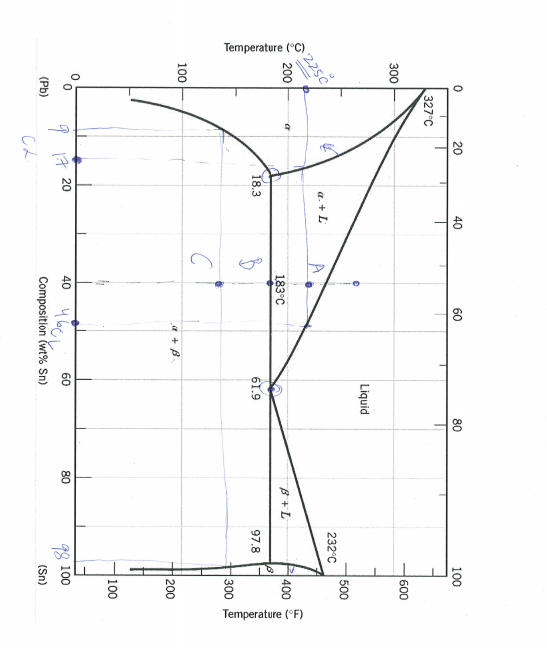
\includegraphics[width=0.66\textwidth]{assets/8edf2f27.png}
    \caption{anotha diagram}
    \label{fig:my_label}
\end{figure}

\paragraph{Example} Pb-Sn phase diagram at 40cot\%



At point A, $C_\alpha = 17, 40, C_L = 46$
\begin{figure}[h!]
	\centering
	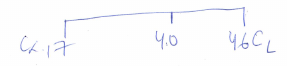
\includegraphics[width=0.36\textwidth]{assets/501239bf.png}
\end{figure}

$N_L = \frac{40-17}{46-17}=$

$w_{\alpha'} = \frac{46-40}{46-17} = $

At point B, $18.3, 40, 61.9$
\begin{figure}[H]
	\centering
	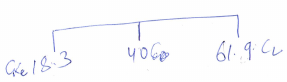
\includegraphics[width=0.36\textwidth]{assets/65a27bc0.png}
\end{figure}

$w_L = \frac{40-18.3}{61.9-18.3} = 49.7\%$

$w_{\alpha_e} = \frac{61.9-40}{61.9-18.3} = 50.3\%$

At point C, $9, 40, 98$

\begin{figure}[h!]
	\centering
	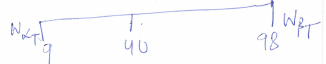
\includegraphics[width=0.66\textwidth]{assets/0ec92081.png}
\end{figure}

$w_{\alpha_T} = \frac{98-40}{98-9}$

$w_{\beta_T} = \frac{40-9}{98-9}$

\section{more phase diagram shit (nov 15)}

The temperature at which the eutectic reaction takes place is called \textbf{eutectic isotherm}.

Any phase that forms above this isotherm is called pre-eutectic (primary).

Any phase that forms below this isotherm is called ``total''.

\subsection{Microstructure development}

The type of microstructure that develops in the material depends on the composition of the alloys.

\subsubsection{Scenario 1}

\begin{figure}[h!]
	\centering
	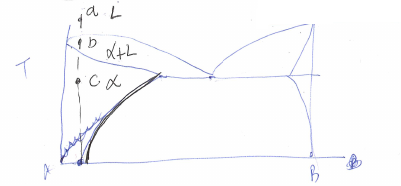
\includegraphics[width=0.66\textwidth]{assets/bfaf63be.png}
\end{figure}   

At A: The material is liquid, predominantely `A' with some B

At B: Solids start to form
\begin{figure}[H]
	\centering
	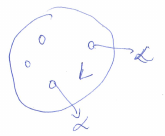
\includegraphics[width=0.16\textwidth]{assets/cf5e3816.png}
\end{figure}

At C: The solid grown and forms $\alpha$ grains, A with a little bit of B
\begin{figure}[h!]
	\centering
	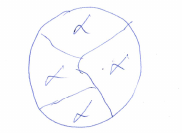
\includegraphics[width=0.16\textwidth]{assets/6a97b795.png}
\end{figure}

\subsubsection{Scenario 2}

\begin{figure}[h!]
	\centering
	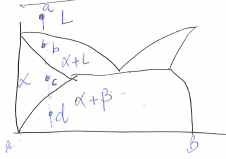
\includegraphics[width=0.66\textwidth]{assets/6c779bcf.png}
\end{figure}

At A: Everything is liquid, matrix is predominately A with some B

At B: We enter a semi-solid region with \textalpha+L
\begin{figure}[h!]
	\centering
	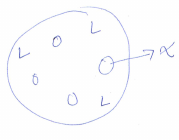
\includegraphics[width=0.16\textwidth]{assets/da3df784.png}
\end{figure}

At C:\begin{figure}[h!]
	\centering
	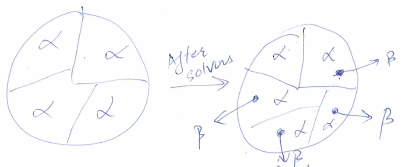
\includegraphics[width=0.46\textwidth]{assets/6584bc34.png}
\end{figure}

At D: 
\begin{figure}[h!]
	\centering
	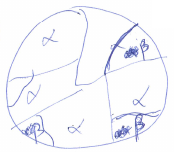
\includegraphics[width=0.16\textwidth]{assets/4ffbff85.png}
\end{figure}

As we cool down, the material enters into $\alpha$ + $\beta$. We need to form $\beta$
\begin{itemize}
    \item $\beta$ forms by re-precipitation from $\alpha$ that existed at higher temperatures.
    \item $\beta$ phase occurs throughout the material.
\end{itemize}

\subsubsection{Scenario 3}

\begin{figure}[H]
	\centering
	\includegraphics[width=0.66\textwidth]{assets/71711602.png}
    \caption{Yet another rough diagram}
    \label{fig:my_label}
\end{figure}

At A: Liquid

A+B: 
\begin{figure}[h!]
	\centering
	\includegraphics[width=0.36\textwidth]{assets/ae08853c.png}

\end{figure}

\begin{itemize}
    \item The material needs to cool and transform from L to $\alpha+\beta$ at a single temperature.
    \item The solid phase must be made of two different phases (chemically different)
    \item These two phases will begin to grow at the same time and form ``lamellae''\\ (\url{https://en.wikipedia.org/wiki/Lamella_(materials)})
\end{itemize}


\subsubsection{Scenario 4}

\begin{figure}[H]
	\centering
	\includegraphics[width=0.66\textwidth]{assets/667f21c8.png}
    \caption{really? Another diagram?}
    \label{fig:my_label}
\end{figure}

At B: 
\begin{figure}[h!]
	\centering
	\includegraphics[width=0.66\textwidth]{assets/9f0f1e02.png}
\end{figure}

The $\alpha$ phase begins to grow and is surrounded by liquid

At C: the liquid solidifies with a eutectic composition forming lamellae.

\section{Fe-C phase diagram (nov 17)}
Iron is the most commonly used metal globally. Construction, machines, etc. all rely on Fe-based systems. Australia is max producer of iron.

\subsection{Terminology}
Iron will transform as it is heated and cooled

It starts as an $\alpha$-iron (BCC)

@ 912 degrees converts to $\gamma$ iron

@ 1294 degrees converts to $\delta$ iron (BCC) `$\delta$ ferrite'

@ 1538 degrees $\delta$ ferrite melts

Majority of Fe-C materials have a composition less than 7 wt\% C

\paragraph{nov 19}

The phase that exists at 6.67wt\% C is called ``Fe$_3$C'' or cementite.

Fe$_3$C is not a solid solution, but it is an intermetallic component with exact stoichiometry.

The amount of C that we can dissolve in Fe depends on the crystal structure of Fe.

\textalpha-Ferrite (BCC): carbon wants to go into the intersticial positions. These are limited only 0.022 wt\% C in \textalpha-ferrite.

\textgamma-Iron(FCC): has a different lattice structure with more open spaces for C to occupy. We can dissolve up to 2.14 wt\% C.

Recall we had a case where liquid transforms into solids

\[L \rightleftharpoons \alpha + \beta \text{ Eutectic reaction}\] 

In Fe-C phase diagram:

\[L \rightleftharpoons \gamma + Fe_3C \text{ Eutectic reaction}\] 

When a solid material transforms into two phases:

\[\gamma \rightleftharpoons \alpha + Fe_3C \text{ Eutectoid reaction}\]

\subsection{Microstructure}

\begin{enumerate}
    \item At eutectoid composition 0.76 wt\% C
    \begin{figure}[h!]
	    \centering
	    \includegraphics[width=0.66\textwidth]{assets/7ada0b1a.png}
    \end{figure}
    
    The combination of \textalpha + Fe\textsubscript{3}C (i.e. lamellar structure) is called ``Pearlite''
    \item Hyper-eutectoid alloy (November 22)
    
    \begin{itemize}
        \item The alloy starts as Austenite (\textgamma)
        \begin{figure}[h!]
	        \centering
	        \includegraphics[width=0.26\textwidth]{assets/63f8c9b2.png}
        \end{figure}
        
        \paragraph{\textgamma-Iron (FCC)} Has a different lattice structure with more open spaces for C to occupy. We can dissolve up to 2.14 wtr C
        
        Recall we had a case (on binary P.D.) when liquid transforms into two solids
        
        \[L\rightleftharpoons \alpha + \beta \text{(eutectic rxn)}\]
        
        In Fe-C P.D.
        
        \[L\rightleftharpoons \gamma + Fe_3C \text{(also eutectic rxn)}\]
        
        When a solid material transforms into two phases:
        
        \[\gamma\rightleftharpoons \alpha + Fe_3C \text{(eutectoid rxn)}\]
        
        As we start cooling the material, we cross into \textgamma+\textalpha\ region
        
        \begin{figure}[H]
        	\centering
        	\includegraphics[width=0.36\textwidth]{assets/9c7e3723.png}
        \end{figure}
        
        \item As we cool the material, we enter the \textgamma\ + Fe$_3$C region, and Fe$_3$C needs to precipitate out
        
        \begin{figure}[h!]
	        \centering
        	\includegraphics[width=0.36\textwidth]{assets/499083ec.png}
        \end{figure}
        
        \item Below the eutectoid temperature: \textgamma\ needs to transform to \textalpha\ + Fe$_3$C
        
        \begin{figure}[h!]
        	\centering
        	\includegraphics[width=0.66\textwidth]{assets/85256a9e.png}
        \end{figure}
        
        \begin{figure}[H]
        	\centering
        	\includegraphics[width=0.66\textwidth]{assets/6d4f2ebd.png}
        	\caption{phase diagram of something}
        \end{figure}
    \end{itemize}
   
\end{enumerate}

\paragraph{Example} Is it possible to have a Cu-Ag alloy in which the mass fraction of $\beta\prime$ and total $\beta$ are 0.68 and 0.925 respectively at 779\si\degree C. Why?

\paragraph{Answer}

\begin{figure}[H]
	\centering
	\includegraphics[width=0.36\textwidth]{assets/03120a3b.png}
\end{figure}

$W_{\beta\prime} = \frac{C_0-71.9}{91.2-71.9} = 0.68$\\
$C_0 = 85 wt\% \text{Ag}$\\
\begin{figure}[h!]
	\centering
	\includegraphics[width=0.36\textwidth]{assets/e2dc5140.png}
\end{figure}
$W_b = \frac{C_0 - 8}{91.2-8} = 0.925$\\
$C_0 = 85wt\%{Ag}$

Since both $C_0$ are equal, the alloy is possible

\paragraph{Example 2} Consider a Mg-Pb alloy with 30 wt\% Pb and 70 wt\% Mg. If we have 11.2 kg of this alloy, at what temperature will we have 7.39kg of $\alpha$ and 3.91 kg of Mg$_2$Pb?

\paragraph{Answer} \begin{align*}
    w_\alpha &= \frac{7.39}{7.39+3.81} = 0.66\\
    w_{Mg_2Pb} &= \frac{3.81}{7.39+3.81} = 0.34
\end{align*}

\begin{figure}[h!]
	\centering
	\includegraphics[width=0.36\textwidth]{assets/300f211e.png}
\end{figure}    

\begin{align*}
    w_\alpha &= \frac{81-30}{81-x} = 0.66\\
    x&= 3.7wt\%\text{Pb}
\end{align*}

\paragraph{Question (Nov 24)} What is the concentration of carbon pf an Fe-C alloy, for which the total ferrite is 0.94 just after crossing the eutectoid temperature?

\paragraph{Answer} \begin{align*}
    w_{\alpha tot} &= \frac{6.7-C_0}{6.7-0.022} = 0.94\\
    C_0 &= 0.42 wt\% C
\end{align*}

\section{Strengthening and grain growth (Nov 26)}

In general, the stronger a material, the less ductile it is
\begin{figure}[h!]
	\centering
	\includegraphics[width=0.66\textwidth]{assets/7ad81afb.png}
	\caption{ductility graph}
\end{figure}

Stronger materials are less likely to allow dislocation movements
\begin{itemize}
    \item Grain size effect
    \begin{itemize}
        \item Smaller grains ideal
    \end{itemize}
    \item Solid solution hardening
    \begin{itemize}
        \item adding alloying elements
    \end{itemize}
    \item Strain hardening
\end{itemize}

\subsection{Grain size effect}
Hall-petch relation:

$\sigma_y = \sigma_0 + \frac{Ry}{\sqrt{d}}$

where $\sigma_y$ is yield stress, $\sigma_0, R_y$ are constants, and $d$ is average grain diameter.

Smaller grains lead to more $\sigma_y$, also lead to more grain boundaries impeding dislocation movement.

\subsection{Solid solution strengthening}

Addition of alloying elements to improve properties

Common in steels:
\begin{itemize}
    \item Boron (B) \textrightarrow\ hardening agent
    \item Chromium (Cr) \textrightarrow\ hardening agent + corrosion resistance
    \item Molybdenium (Mo) \textrightarrow\ Grain refinement (improves toughness)
    
\end{itemize}

\subsection{Precipitation hardening/age hardening}
Heat treatment process to produce uniform distribution of impurity phase (precipitates) which inhibit movement of dislocations.

\section{Strain hardening (Nov 29)}
Ductile materials become stronger as they are plastically deformed

$ \%CW = \frac{A_0 -Ad}{A_0}\times 100\%$

$A_0$ original area, $Ad$ deformed area.

This effect is due to dislocation interactions
\begin{itemize}
    \item As metals physically deform, dislocation merge or form new ones.
    \item Therefore, density of dislocations within a material increases
    \item These dislocations typically have a repulsive interaction
\end{itemize}

\section{Recrystallization}

Formation of new stress free grains, (equiaxed grains same. ... idk what she wrote here

\section{Corrosion in metals (dec 1)}

In metals, material degradation occurs by two mechanisms:
\begin{enumerate}
    \item Dissolution: material loss due to corrosion and scaling of the material
    \item Oxidation: formation of oxides on the material, usually resulting in weight gain
\end{enumerate}
For metals, corrosion/oxidation is driven by transfer of e\textsuperscript{-1}s. If e\textsuperscript{-1}s can be stopped or diverted, then corrosion will stop.

Metals readily give up electrons from their valence shell

$Fe \rightarrow Fe^{2+} + 2e^{-}$

So the Fe\textsuperscript{2+} is a deficient atom (it is not in equilibrium) and it will be waiting to receive electrons. 

Oxidation reaction: 
\[M \rightarrow M^{n+} + ne^{-}\]

This reaction takes place at an anode and so it is called an anodic reaction

Reduction reaction: 
\[M^{n+} + ne^- \rightarrow M\]

The adsorption of e\textsuperscript{-} is called reduction reaction. (cathode)

Different combination of metals have different tendencies

The driving potential for corrosion is given by the voltage potential between the two metals

%some fucking diagram with an external circuit, iron and copper
\begin{figure}[h!]
	\centering
	\includegraphics[width=0.66\textwidth]{assets/84bf8c79.png}
	\caption{electrodes woohoo}
\end{figure}

We can develop a standard electrode

Called a standard hydrogen electrode (SHE)

The oxidation and reduction is the fundamental principle of batteries

\subsection{Standard electrode half cell (Dec 3)}

The standard electrode is made of platinum with 1 M of H\textsuperscript{+} ions.

\begin{figure}[h!]
	\centering
	\includegraphics[width=0.46\textwidth]{assets/7b0c4229.png}
	\caption{standard platinum electrode}
\end{figure}

We can use this to compare the oxidation and reduction potentials of different metals.

M\textsubscript{1} oxidizes: $M_1\rightarrow M_1^{n+}+ne^{-}-v_1^0$

M\textsubscript{2} reduces: $M_2^{n+}+ne^-\rightarrow M_2+v_2^0$

\[M_1+M_2^{n+} \rightarrow M_1^{n+} + M_2\]

The materials in a galvanic series will have a positive or negative value with respect to SHE.

The overall cell potential: $\Delta V^0 = V_2^0 - V_1^0$

\begin{figure}[h!]
	\centering
	\includegraphics[width=0.66\textwidth]{assets/fffedf23.png}
	\caption{galvanic series}
\end{figure}

\begin{figure}[h!]
	\centering
	\includegraphics[width=0.66\textwidth]{assets/0c092313.png}
	\caption{The standard emf series}
	\label{anotherseries}
\end{figure}

$\Delta V_0$ should be positive for the reaction to proceed in the assumed direction.

If $\Delta V_0$ is negative, then reverse the assumed reaction.

Changing the temperature and concentration of ions in the solution will affect the cell voltage.

$\Delta V = (V_2^0 - V_1^0) - \frac{RT}{nF}\ln\left[\frac{M_1^{n+}}{M_2^{n+}}\right]$

Where $R$ is the gas constant and is equal to 8.3145, $F$ is Faraday's constant and is 96500, $n$ is number of elections, and $T$ is temperature.

Inside the ``[ ]" are concentrations of solutions with ions.

$V_1^0$ and $V_2^0$ are voltages for the half cell reactions.

At room temperature:

\[\Delta V = (V_2^0 - V_1^0) - \frac{0.0592}{n}\log\frac{[M_1^{n+}]}{[M_2^{n+}]}\]

\paragraph{Example} We have a battery cell with pure cadmium immersed in a $2\times10^{-3}$M solution of Cd\textsuperscript{2+}. The second electrode is pure iron immersed in 0.4 M solution of Fe\textsuperscript{2+} ions. What is the voltage on this cell?

\begin{align*}
    Fe &\rightarrow Fe^{2+} + 2e^-\\
    V_0 &= -0.440\\
    Cd^{2+} + 2e^- &\rightarrow Cd\\
    V_0 &= -0.403
\end{align*}

The voltage values are from the table above in Figure \ref{anotherseries}.

\begin{align*}
    \Delta V &= (V_2^0 - V_1^0) - \frac{0.0592}{n}\log\frac{[Fe^{2+}]}{[Cd^{2+}]}\\
    &= (-0.403 - (-0.440)) - \frac{0.0592}{2}\log\left(\frac{0.4}{2\times10^{-3}}\right)\\
    &= -0.031\si\volt
\end{align*}

The above working is wrong, since the final voltage should not be negative. We assumed the iron was losing electrons.

\begin{equation*}
    Fe^{2+} + Cd \rightarrow Fe + Cd^{2+}
\end{equation*}

Since \textDelta V is negative, the reaction actually proceeds in the opposite direction than what was assumed. In fact, the cadmium is oxidized, iron is reduced.

\subsection{Corrosion Rate (Dec 6)}
In real life, electrode potentials will not always be achieved, because of material inhomogeneity and difficulties in perfectly controlling the electrical circuit. 

More so, the emf values (from the table) tells us the tendency of 2 materials to react.

To quantify; corrosion rate can be expressed as 

$CPR = \frac{KW}{\rho At}$

Where $K$ is a constant (87.6), $W$ is amount of material that is lost (mg), $t$ is time (hour), $A$ is exposed area (cm\textsuperscript{2}), and $\rho$ is density (g/cm\textsuperscript{3}).

\paragraph{Example} A thick sheet of steel of 400cm\textsuperscript{2} is exposed to air near the ocean. After one year of sitting there, it has lost 375 grams due to corrosion. What is the corrosion rate?

\paragraph{Answer} 
\begin{align*}
    CPR &= \frac{KW}{\rho At}\\
    &= \frac{87.6(375\si\g \times 1000)}{7.9\si{\g\per\cubic\cm} (400\si{\cm\squared})(24\times365 \text{days})}\\
    &= 1.2\text{mm/year}
\end{align*}

We can measure how much current is generated when a material is corroding.

We can measure the current per surface area of a material:
\[r = \frac{i}{nF}\]

where $i$ is current, $F$ is faraday's constant, and $n$ is number of electrons involved.

\textbf{our notes are fucking done}

\end{document}
